\section{Peeling decoder}
\subsection{LDPC Code}

\begin{frame}\frametitle{Tanner Graph - LDPC Code}
\begin{columns}

\column{0.45\textwidth}
\begin{defn}{Parity-Check Matrix}
\centering
\begin{align*}
H=
\begin{pmatrix}
1 & 0 & 1 & 1 & 0 & 0\\
1 & 1 & 0 & 0 & 1 & 0\\
0 & 1 & 1 & 0 & 0 & 1
\end{pmatrix}
\end{align*}
\vspace{6ex}
\begin{align*}
\text{LDPC Code } \mc{C}=\{x: H\odot x=0 \}
\end{align*}
\end{defn}

\pause

\column{0.45\textwidth}
\begin{defn}{Tanner Graph}
\centering
\vspace{0.6cm}
\resizebox{\textwidth}{!}{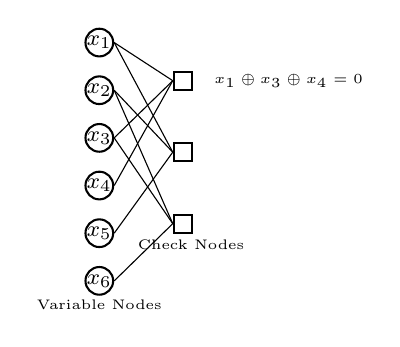
\begin{tikzpicture}
\def\horzgap{7ex}; %Horizontal gap between nodes/levels
\def \gapVN{4ex}; %vertical gap between variable nodes
\def \gapCN{6ex}; %Horizontal gap between check nodes
\def\nodewidth{1.5ex};

\def \textoffs{1ex}; %Offset for writing text east of a node
%\def\nodewidthA{0.05in};
%\def \edgewidth{0.02in};
%\def\ext{0.2in};
`
\def \n{8};
\def\ldeg{2};
\def \m {4};
\def\rdeg{3};

\def\langle{40};%120 degrees/3
\def\langle{20};%120 degrees/6

\tikzstyle{check} = [rectangle, draw, line width=0.75pt, inner sep=0mm, minimum height=\nodewidth, minimum width=\nodewidth]
\tikzstyle{bit} = [circle, draw,line width=0.75pt, inner sep=0mm, minimum size=\nodewidth]

                          
\foreach \vn in {1,...,6}{
 \node[bit] (vn\vn) at (0,-\vn*\gapVN) {\footnotesize $x_{\vn}$};
}


\foreach \cn in {1,...,3}{
\node[check] (cn\cn) at (\horzgap,-0.2*\gapCN-\cn*\gapCN) {};
}

\path (cn1.east)++(\textoffs,0) node ()[anchor=west] {\tiny{$x_1\oplus x_3\oplus x_4=0$}};

%\draw (vn6.east)--(cn4.west);
%\draw (vn3.east)--(cn4.west);
%\draw (vn1.east)--(cn4.west);

%\draw(vn2.east)--(cn3.west);
%\draw (vn4.east)--(cn3.west);
%\draw(vn5.east)--(cn3.west);

\draw (vn2.east)--(cn3.west);
\draw (vn3.east)--(cn3.west);
\draw  (vn6.east)--(cn3.west);

\draw (vn1.east)--(cn2.west);
\draw (vn2.east)--(cn2.west);
\draw (vn5.east)--(cn2.west);

\draw (vn1.east)--(cn1.west);
\draw (vn3.east)--(cn1.west);
\draw (vn4.east)--(cn1.west);

\node () at (0,-6.5*\gapVN){\tiny Variable Nodes};
\node () at (1.1*\horzgap,-3.5*\gapCN){\tiny Check Nodes};

\end{tikzpicture}}
\end{defn}

\end{columns}
\end{frame}

%--------------------------12314yoi34u9123092u308912------------------------------
\subsection{Decoder-BEC Channel}
\begin{frame}
\frametitle{Iterative peeling process}
\begin{columns}
\column{0.4\textwidth}
\begin{align*}
x_1\oplus x_3\oplus x_4&=0\\
x_1\oplus x_2\oplus x_5&=0\\
x_2\oplus x_3\oplus x_5&=0
\end{align*}

\vspace{0.2cm}
\centering
\only<2->{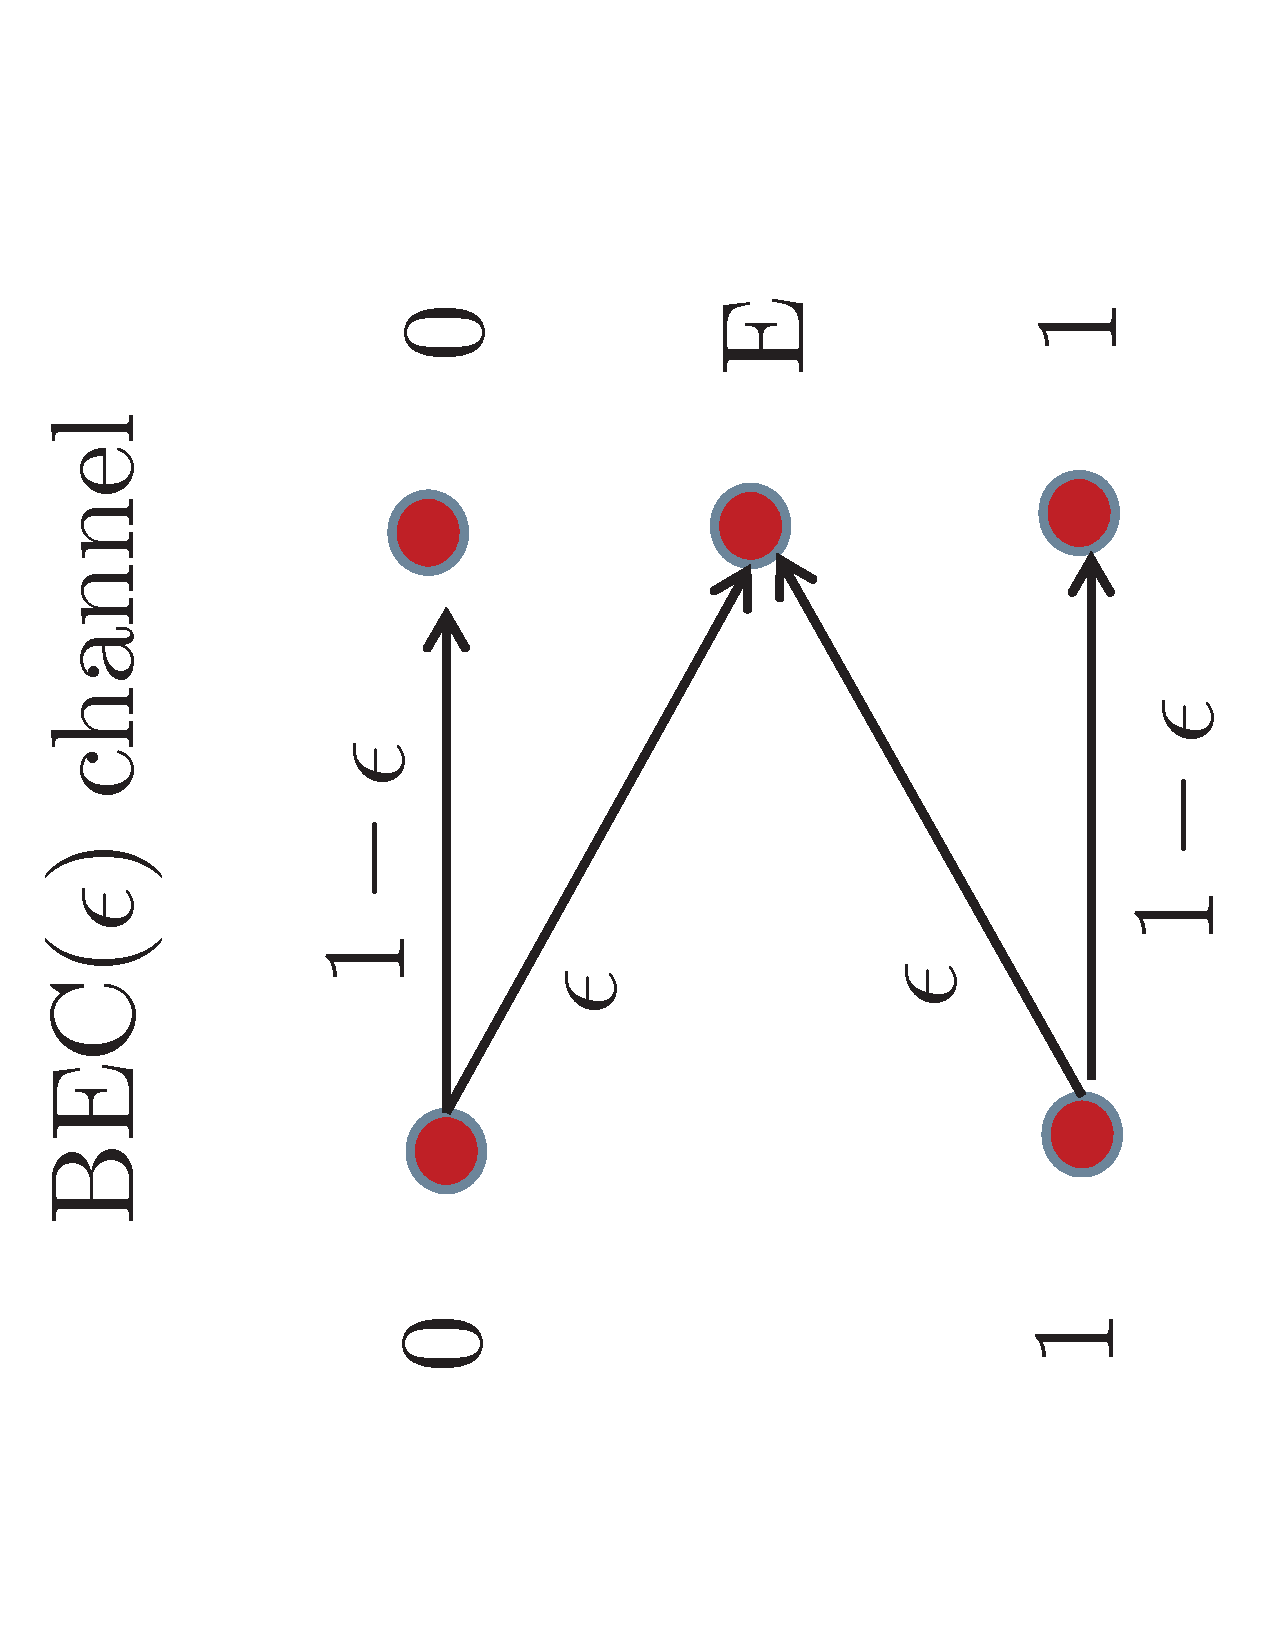
\includegraphics[scale=0.15,angle=270]{\figpath/BECchannelmodel.pdf}}

\column{0.6\textwidth}
\resizebox{0.9\textwidth}{!}{\pgfdeclarelayer{background}
\pgfdeclarelayer{foreground}
\pgfdeclarelayer{m-f}
\pgfdeclarelayer{main}

\pgfsetlayers{background,foreground}
\colorlet{LightBlue}{blue!10!white}
\colorlet{DarkBlue}{blue!80!white}

\begin{tikzpicture}[scale=1.0]
\clip (-0.15in,0.15in) rectangle (1.3in,-2.5in);

\def\n     {6}   % #-Variable nodes
\def\m     {3}  % #-Check nodes
\def\nodewidth{0.15in}
\def\nodegapVN{0.3in}
\def\nodegapCN{0.5in}

\tikzstyle{check} = [rectangle, draw, text centered, thick, fill=red,
                          minimum height=\nodewidth, minimum width=\nodewidth]
\tikzstyle{bit} = [circle, draw, text centered, thick, fill=LightBlue,
                          radius=0.5*\nodewidth]
\tikzstyle{bitpeeled} = [circle, draw, text centered, thick, fill=DarkBlue,
                          radius=0.5*\nodewidth]

\begin{pgfonlayer}{background}
%\draw[gray,step=0.5in] (-0.15in,0.15in) grid (1.5in,-2.5in);
\foreach \vn in {1,...,\n}{
  \node[bit] (vn\vn) at (0,-\vn*\nodegapVN) {};
 }

 \foreach \cn in {1,...,\m}{
  \node[check] (cn\cn) at (1in,-\cn*\nodegapCN) {};
 }
\end{pgfonlayer}



\begin{pgfonlayer}{foreground}

%Text to left of VN
\only<1>{
\foreach \vn in {1,...,\n}{
  \node[left] (nodetxt) at (vn\vn.west) {\normalsize{$x_\vn$}};
 	}  	
}

\only<2-8>{
\foreach \vn/\txt in {2/1,4/1,5/0}{
\node[left] (nodetxt) at (vn\vn.west) {\normalsize{\txt}};
 	}	
}

\only<2-3>\node[left] (nodetxt) at (vn1.west) {\normalsize{E}};
\only<2-5>\node[left] (nodetxt) at (vn3.west) {\normalsize{E}};
\only<2-7>\node[left] (nodetxt) at (vn6.west) {\normalsize{E}};


\only<4-8>\node[left] (nodetxt) at (vn1.west) {\normalsize{E=1}};
\only<6-8>\node[left] (nodetxt) at (vn3.west) {\normalsize{E=0}};
\only<8>\node[left] (nodetxt) at (vn6.west) {\normalsize{E=1}};

%Edges
\uncover<1-2>{
\foreach \vn/\cn in {2/2,2/3,4/1,5/2}{
 \draw[thick] (vn\vn.east)--(cn\cn.west);
  }
}

\only<1-3>\draw[thick] (vn1.east)--(cn2.west);
\only<1-4>\draw[thick] (vn1.east)--(cn1.west);

\only<1-5>\draw[thick] (vn3.east)--(cn1.west);
\only<1-6>\draw[thick] (vn3.east)--(cn3.west);

\only<1-5>\draw[thick] (vn3.east)--(cn1.west);
\only<1-6>\draw[thick] (vn3.east)--(cn3.west);

\only<1-7> \draw[thick] (vn6.east)--(cn3.west);

%% Peeled bits color
\uncover<3-8>{
  \foreach \vn in {2,4,5}{
    \node[bitpeeled] () at (vn\vn) {};
    }
  }
 \only<4-8>\node[bitpeeled] () at (vn1) {};
 \only<6-8>\node[bitpeeled] () at (vn3) {};
  \only<8>\node[bitpeeled] () at (vn6) {};

%Check node values
\only<2,5,6,7,8> \node[right] (nodetxt) at (cn1.east) {\normalsize{0}};
\only<3,4> \node[right] (nodetxt) at (cn1.east) {\normalsize{1}};

\only<2,4,5,6,7,8> \node[right] (nodetxt) at (cn2.east) {\normalsize{0}};
\only<3> \node[right] (nodetxt) at (cn2.east) {\normalsize{1}};

\only<2,6,7,8> \node[right] (nodetxt) at (cn3.east) {\normalsize{0}};
\only<3,4,5> \node[right] (nodetxt) at (cn3.east) {\normalsize{1}};



%% Text at the bottom
\only<1> \node[minimum width=10cm] (txt) at (0.5in,-7*\nodegapVN) {Tanner Graph};
\only<2> \node[minimum width=10cm] (txt) at (0.5in,-7*\nodegapVN) {Received block};
\only<3> \node[minimum width=10cm] (txt) at (0.5in,-7*\nodegapVN) {Peeling Step 1};
\only<4-5> \node[minimum width=10cm] (txt) at (0.5in,-7*\nodegapVN) {Peeling Step 2};
\only<6-7> \node[minimum width=10cm] (txt) at (0.5in,-7*\nodegapVN) {Peeling Step 3};
\only<8> \node[minimum width=10cm] (txt) at (0.5in,-7*\nodegapVN) {Peeling Step 4};

\end{pgfonlayer}
\end{tikzpicture} }
\end{columns}
\end{frame}

%--------------------------12314yoi34u9123092u308912------------------------------
\begin{frame}\frametitle{Threshold behavior}
\begin{columns}
\column{0.45\textwidth}
\begin{defn}{Threshold behavior}
\begin{itemize}
\item $N$-variable nodes, $m$-check nodes %$\epsilon$-erasure probability
\item If $m=\alpha N$ scales linearly, $\exists \alpha^{*}$
\begin{align*}
\lim_{N\rightarrow \infty}\Pr(\mc{E})=0 ~~ \text{ if }\alpha>\alpha^*
\end{align*}
\item $\Pr(\mc{E})>0$ if $\alpha<\alpha^*$
\end{itemize}
\end{defn}

\pause

\column{0.55\textwidth}
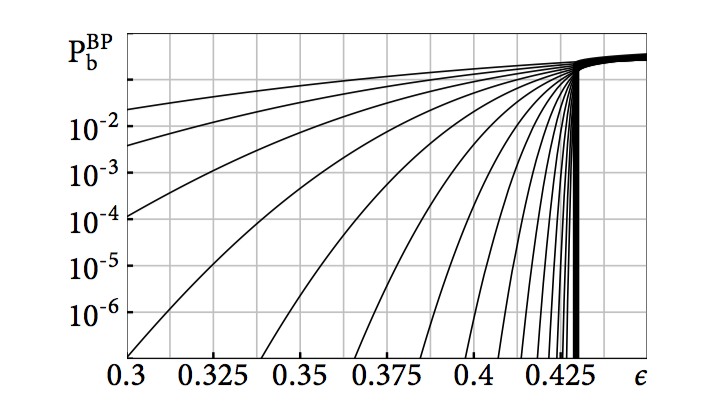
\includegraphics[width=\textwidth]{\figpath/BEC_MCT.png}
\begin{itemize}
\item $\Pr(\mc{E})$ for (3,6) d.d. for $N=2^i, i=6,\ldots,20$.  $m=N/2$
\end{itemize}

\end{columns}
\end{frame}

%--------------------------12314yoi34u9123092u308912------------------------------
\begin{frame}\frametitle{General framework}
\begin{columns}
\column{0.4\textwidth}
\resizebox{\textwidth}{!}{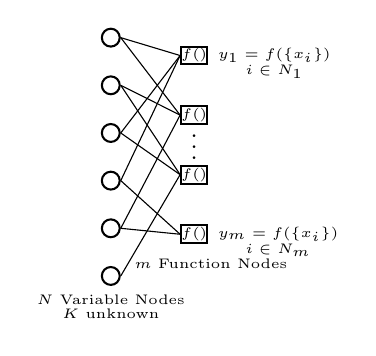
\begin{tikzpicture}
\def\horzgap{7ex}; %Horizontal gap between nodes/levels
\def \gapVN{4ex}; %vertical gap between variable nodes
\def \gapCN{5ex}; %Horizontal gap between check nodes
\def\nodewidth{1.5ex};

\def \textoffs{1ex}; %Offset for writing text east of a node
%\def\nodewidthA{0.05in};
%\def \edgewidth{0.02in};
%\def\ext{0.2in};
`
\def \n{8};
\def\ldeg{2};
\def \m {4};
\def\rdeg{3};

\def\langle{40};%120 degrees/3
\def\langle{20};%120 degrees/6

\tikzstyle{check} = [rectangle, draw, line width=0.75pt, inner sep=0mm, minimum height=\nodewidth, minimum width=\nodewidth]
\tikzstyle{bit} = [circle, draw,line width=0.75pt, inner sep=0mm, minimum size=\nodewidth]

                          
\foreach \vn in {1,...,6}{
 \node[bit] (vn\vn) at (0,-\vn*\gapVN) {};
}


\foreach \cn in {1,...,4}{
\node[check] (cn\cn) at (\horzgap,-0.1*\gapCN-\cn*\gapCN) {\tiny{$f()$}};
}

\path (cn2)++(0,-0.4*\gapCN) node () {\small{$\vdots$}};

\path (cn1.east) node[anchor=west] (ytexta) {\tiny{$y_1=f(\{x_i\})$}};
\path (ytexta) node[anchor=north] () {\tiny{$i\in\mc{N}_1$}};

%\path (cn4.east) node[anchor=west] () {\tiny{$y_m=f(\{x_i,i\in\mc{N}_m\})$}};

\path (cn4.east) node[anchor=west] (ytextb) {\tiny{$y_m=f(\{x_i\})$}};
\path (ytextb) node[anchor=north] () {\tiny{$i\in\mc{N}_m$}};


\draw (vn4.east)--(cn4.west);
\draw  (vn5.east)--(cn4.west);

\draw (vn2.east)--(cn3.west);
\draw (vn3.east)--(cn3.west);
\draw  (vn6.east)--(cn3.west);

\draw (vn1.east)--(cn2.west);
\draw (vn2.east)--(cn2.west);
\draw (vn5.east)--(cn2.west);

\draw (vn1.east)--(cn1.west);
\draw (vn3.east)--(cn1.west);
\draw (vn4.east)--(cn1.west);

%\node[text width=1.5cm] () at (0,-6.5*\gapVN){\tiny $N$ Variable Nodes $K$ unknown};
\node[align=left] () at (0,-6.5*\gapVN){\tiny $N$ Variable Nodes};
\node[align=left] () at (0,-6.8*\gapVN){\tiny $K$ unknown};
\node () at (1.2*\horzgap,-4.6*\gapCN){\tiny $m$ Function Nodes};

\end{tikzpicture}}

\column{0.6\textwidth}
\begin{itemize}
\item Need to recover $K$ unknowns$/N$ variables
\item We know values of $m$ functions $y_1,\ldots,y_m$
\item via peeling decoder, $m=cK$ sufficient {\tiny ($c>1$)}
\end{itemize}
\pause
\vspace{5ex}
\begin{itemize}
\item $c$ depends on the d.d of the graph, can be evaluated analytically via DE
\item $f$ amenable for peeling
\end{itemize}

\end{columns}
\end{frame}

